\section{Decision Maker Gadget}
When talking in a group of people it is sometimes necessary to take a decision about a specific aspect. The easiest way to achieve this is by talking, and Wave with real time communication and editing common documents makes this easy. But this way it might be difficult to easily differentiate all the different options, see who agrees with each one of the options, or quickly decide one. This extension allows every participant to choose an option or add new options to the decision. Participants are also able to quickly see who voted each option along with their user avatar images. This features accompanied by Wave's style of communication make consensus and decision making easier.

\label{subsec:decision_soa}
\subsection{State of the Art}
Because of the nature of Wave, decision making is a very important and basic, so there has been several gadgets made regarding that. It also easily explores all the basic possibilities that the Gadgets API provides. Figures \ref{fig:poll} and \ref{fig:consensuall} show two of them: The first one is Poll by Eric Williams, focused on showing statistics about the results, maybe useful when there is a high amount of votes. The second one is Consensuall by Antonio Tenorio, focused on sharing the personal opinion of each voter about an issue and reaching consensus on it.\\[.2cm]
\begin{figure}[H]
  \center
    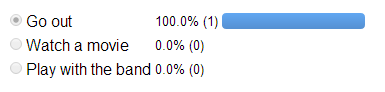
\includegraphics[keepaspectratio, scale=0.7]{Media/Captures/Extensions/DecisionGadgets/other.png}
  \caption{Poll}
  \label{fig:poll}
\end{figure}
\begin{figure}[h]
  \center    
    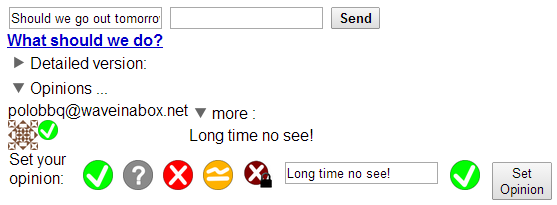
\includegraphics[keepaspectratio, scale=0.7]{Media/Captures/Extensions/DecisionGadgets/consensuall.png}
  \caption{Consensuall}
  \label{fig:consensuall}
\end{figure}
Decision Maker Gadget falls in between both of them by letting people add their own answers, see a representation of the votes and who personally voted for each.

\subsection{Results}
Decision Maker Gadget is a gadget that can be inserted anywhere in a blip. A title is chosen for the issue at hand, and then different options answering that title can be inserted by anyone who sees the gadget, not only the creator. One of the decisions can be instantly chosen by clicking on it.
\begin{figure}[H]
  \center
    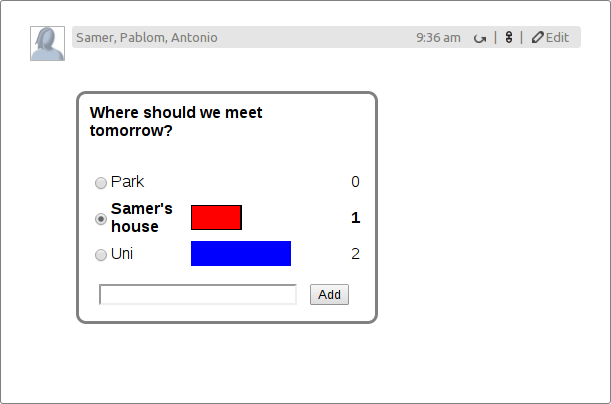
\includegraphics[keepaspectratio, scale=0.4]{Media/Captures/Extensions/DecisionMakerGadget.png}
  \caption{Decision Maker Gadget}
  \label{fig:decision_maker_gadget}
\end{figure}
When there have been decisions chosen by different participants, hovering the mouse over the number of votes on the right will show the names and pictures of the participants that voted for it, as represented in Figure \ref{fig:decision_maker_votes}. Names and pictures are taken from their Wave profile.
\begin{figure}[H]
  \center
    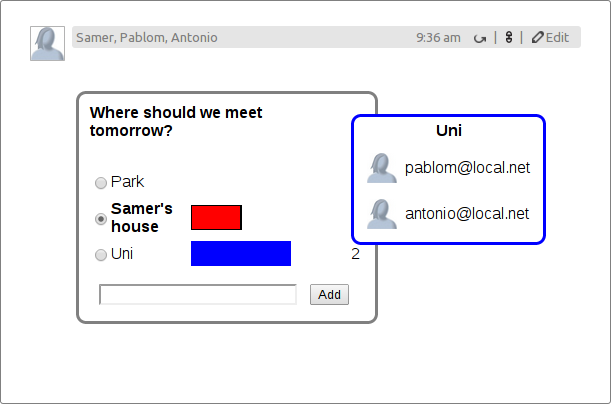
\includegraphics[keepaspectratio, scale=0.4]{Media/Captures/Extensions/DecisionMakerGadget_votes.png}
  \caption{Decision Maker Voters}
  \label{fig:decision_maker_votes}
\end{figure}
This gadget also relates to the structure shown in Figure \ref{fig:gadget_classes}. The GinModule is the DecisionMakerGinModule, the Composite is the DecisionMakerMainPanel, and the Messages class is represented by the class DecisionMakerMessages. This gadget is slightly more complex than the Creative Commons one, so the class diagram with its specifics is shown in Figure \ref{fig:decision_maker_diagram}.
\begin{figure}[H]
  \center
    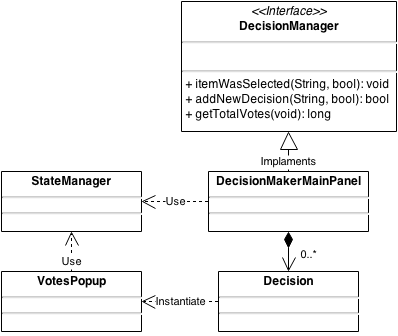
\includegraphics[keepaspectratio, scale=0.5]{Media/Diagrams/Gadget/DecisionMaker.png}
  \caption{UML Class Diagram, Decision Maker}
  \label{fig:decision_maker_diagram}
\end{figure}
The interface DecisionManager is extended. It is meant to represent all that can be done with the decisions: select one, add a new decision, and get the total votes of one specific decision. The DecisionMakerMainPanel implements it, and is also the container for all the decisions. A decision represents one of the options that can be chosen, and generates the Popup showing who voted for it. A StateManager is also used to handle everything related to the Wave's state.\\[.2cm]
There are three different types of entries in the Wave's state:
\begin{itemize}
  \item Count of votes: There is one entry of this kind for each decision. To identify which decision this entry is for, the title of the decision is stored as a key. Therefore, the decision titles have to be unique. The value of this entry is the amount of votes that decision has, making it quick to retrieve the amount and show the vote count.
  \item Voters: Again, one entry for each decision and the title of the decision as an unique identifier. The value is a list of all the people that voted for that decision. As the state is only able to store a string, the list is like \verb+|user1@kune.cc|user2@kune.cc|user3@kune.cc|+. This entry is used to know if a particular user has voted for a decision, and to fill the information inside the votes popup.
  \item Title: There is one single entry for each gadget. The value of this entry is the name of the decision to be taken. Used to fill the title after it has been set.
\end{itemize}
\subsection{Conclusions and Future Work}
There are already several alternatives for decision making, each one with their unique way of doing things, and there is certainly already one suitable for every need, and Decision Maker doesn't innovate in almost any aspect. This alternative has limitations though: There is no option for multi-choice answers, no way of editing the title after being created, and the list of votes can get a little uncomfortable to see after lots of votes have been made. Multi-choice answers would put this gadget closer to a consensus tool, and being able to block options would make the divergence among opinions more visible.
